% ----------------------------------------------------------
% Ajuda.Ai
% ----------------------------------------------------------
\chapter{Ajuda.Ai}

Falando sobre o sistema em si.

\section{Arquitetura}

Bla bla bla alguma coisa sobre arquitetura.

\begin{figure}[H]
  \caption{\label{fig_circulo}Arquitetura do Ajuda.Ai, versão 0.2}
  \centering
  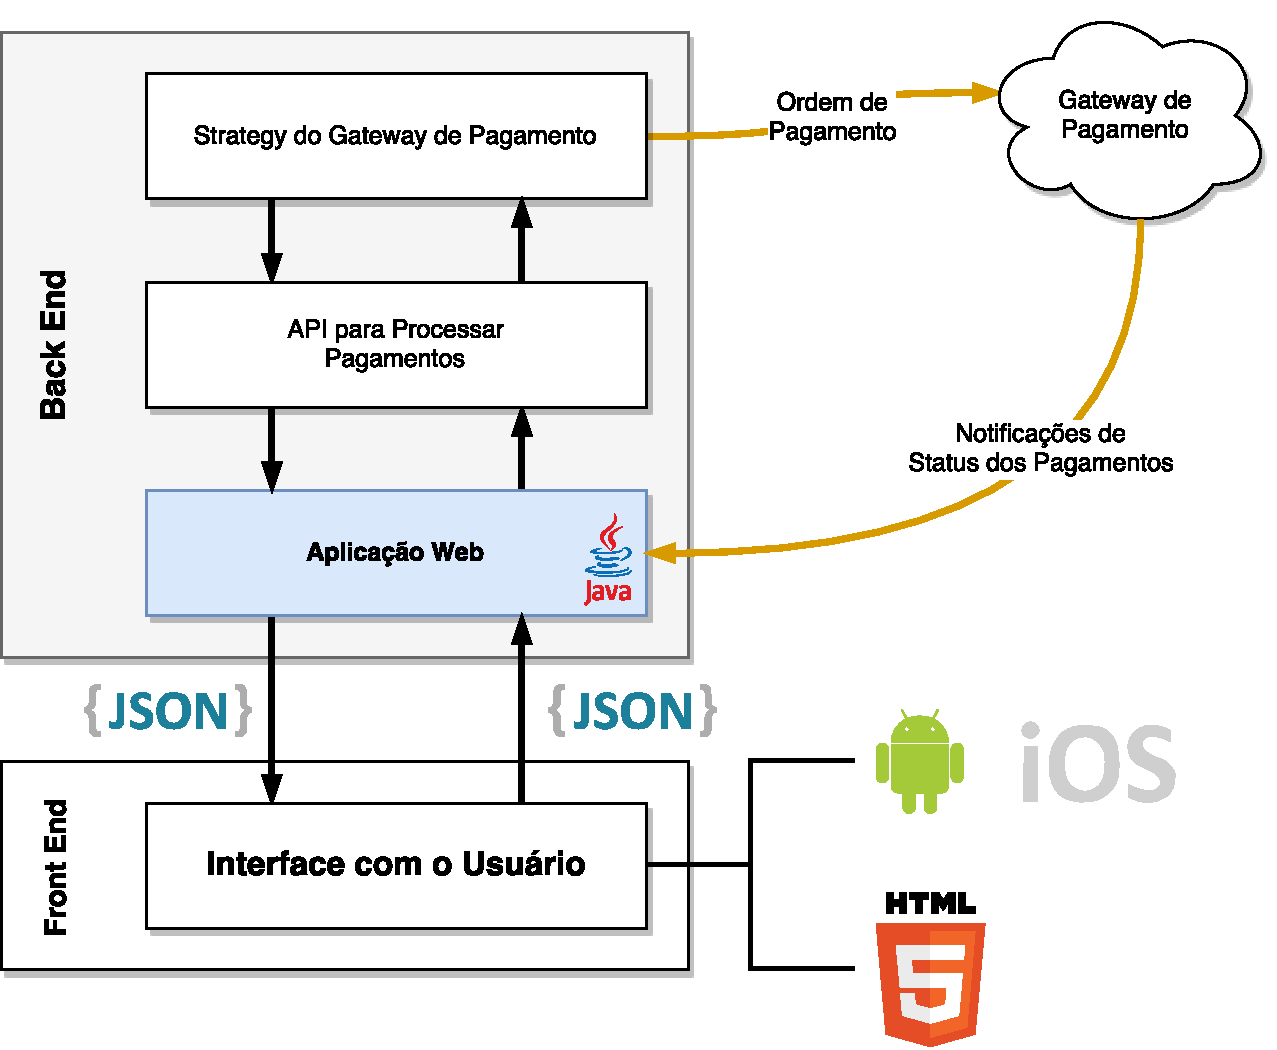
\includegraphics[scale=0.7]{imagens/AjudaAi-Arquitetura-3.pdf}
  \legend{Fonte: Elaborado pelo Autor}
\end{figure}

\subsection{Coisas Sobre o Sistema}

Não sei onde incluir essas coisas, então estou incluindo aqui.

\subsection{Uso do REST}

O sistema usa uma arquitetura REST Web para tornar possível uma completa separação da interface com o usuário, que pode ser feita em HTML5 ou como aplicativos para dispositivos móveis.

Essa arquitetura é recomendada pela W3C\footnote{World Wide Web Consortium, consórcio de empresas e profissionais que buscam padronizar a WWW} em \cite{booth2004webservices}, que define REST Web como ``um subconjunto da WWW (baseado em HTTP) onde agentes provêm semânticas uniformes para interfaces ao contrário de interfaces arbritrárias ou específicas de uma aplicação, e manipulam recursos apenas pela troca de representações.''

\subsection{Diferencial: Suporte a vários Gateways diferentes. Uso de Design Patterns}

Um dos diferenciais do Ajuda.Ai é o suporte a diferentes gateways de pagamento. Isso dá flexibilidade a instituição para usar o gateway mais adequado a mesma. Para implementação foi utilizado o Padrão de Projeto de Software Strategy. Este Padrão de Projeto é definido por uma família de algoritmos encapsulados e que podem ser trocados dentro da família de objetos.

\begin{figure}[H]
	\caption{\label{fig_uml_strategy}Estrutura dos Processadores de Pagamento}
    \centering
	\begin{tikzpicture}
		\umlclass[type=interface]{PaymentProcessor}{}{
			+ createPayment() : Payment \\
            + processEvent() : PaymentEvent}
        \umlclass[x=-3.5, y=-4]{MoipPaymentProcessor}{}{
			+ createPayment() : Payment \\
            + processEvent() : PaymentEvent}
        \umlclass[x=3.5, y=-4]{PagSeguroPaymentProcessor}{}{
			+ createPayment() : Payment \\
            + processEvent() : PaymentEvent}
        \umlsimpleclass[x=-3, y=3]{InstitutionSiteController}
        \umlsimpleclass[x=3, y=3]{TransactionNotificationsController}
        \umlcompo{InstitutionSiteController}{PaymentProcessor}
        \umlcompo{TransactionNotificationsController}{PaymentProcessor}
        \umlimpl{MoipPaymentProcessor}{PaymentProcessor}
        \umlimpl{PagSeguroPaymentProcessor}{PaymentProcessor}
  \end{tikzpicture}
  \legend{Fonte: Elaborado pelo Autor}
\end{figure}

Cada gateway de pagamento suportado implementa a interface PaymentProcessor. Esta interface tem dois métodos:

\begin{itemize}
  \item \textbf{createPayment()}: Cria uma ordem de pagamento junto ao gateway de pagamento. Este método tem liberdade de redirecionar o usuário para o sistema do gateway (MoIP e a maioria dos gateways nacionais) ou enviar algum pedaço de informação, como JSON, como resposta ao usuário (PayPal + JavaScript para pagamento na própria página). Este método deve retornar um objeto Payment para ser persistido a fim de acompanhar o andamento do pagamento;

  \item \textbf{processPayment()}: Gateways de pagamento enviam requisições de volta ao sistema informando sobre o status de um determinado pagamento feito na plataforma deles. Este método é encarregado de processar essas mudanças de estado no pagamento. Este método deve retornar um objeto PaymentEvent que indica de forma padronizada o que aconteceu com este pagamento.
\end{itemize}

Ao criar uma ordem de pagamento através de \textbf{createPayment()} a classe que a criou retorna um objeto Payment para ser persistido. Este objeto, além de padronizar as informações relevantes dos pagamentos, guarda consigo a estratégia (serviço de pagamento) utilizada para criar a ordem de pagamento. Essa informação é usada futuramente quando o sistema recebe uma notificação de estado de pagamento.

Uma vantagem da utilização do padrão Strategy é que diferentes usos de um mesmo gateway podem ser facilmente implementados. Por exemplo, o gateway MoIP oferece várias formas para criar ordens de pagamento. Três delas são interessantes para o que o Ajuda.Ai propõe:

\begin{itemize}
\item \textbf{Ordem de pagamento via e-mail:} O MoIP envia um e-mail para o usuário onde, na conveniencia do mesmo, ele tem 30 dias para efetuar o pagamento da forma como preferir;
\item \textbf{Check-out Clássico:} O usuário é redirecionado para o Gateway onde ele selecionará forma de pagamento e fará todo o processo de pagamento antes de voltar ao Ajuda.Ai;
\item \textbf{Check-out Transparente:} O usuário preenche tudo no próprio sistema o qual junto ao gateway e através de webservices faz uma ordem de pagamento e processamento de pagamento;
\end{itemize}

\subsection{Processo de como acontece um Pagamento nos Gateways}

Um diagrama UML de sequencia que demonstra como acontece um pagamento nos gateways.

\begin{figure}[H]
	\caption{\label{fig_uml_gateway1}Processo Comum de um Pagamento via Gateway de Pagamento}
    \centering
    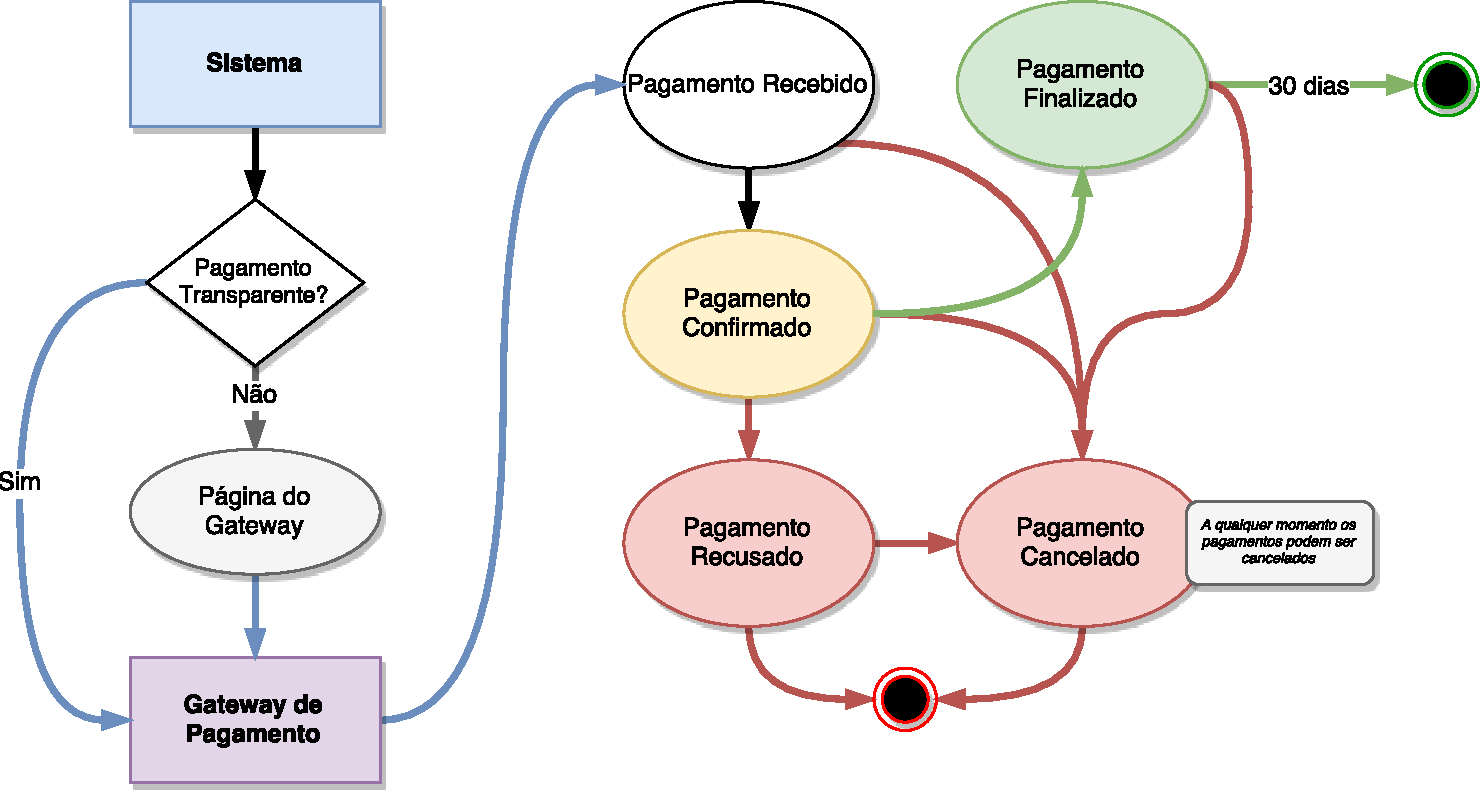
\includegraphics[scale=0.58]{imagens/Processo_Gateway_01.pdf}
    \legend{Fonte: Elaborado pelo Autor}
\end{figure}

\begin{figure}[H]
	\caption{\label{fig_uml_gateway2}Processo Comum de um Pagamento via Gateway de Pagamento}
    \centering
    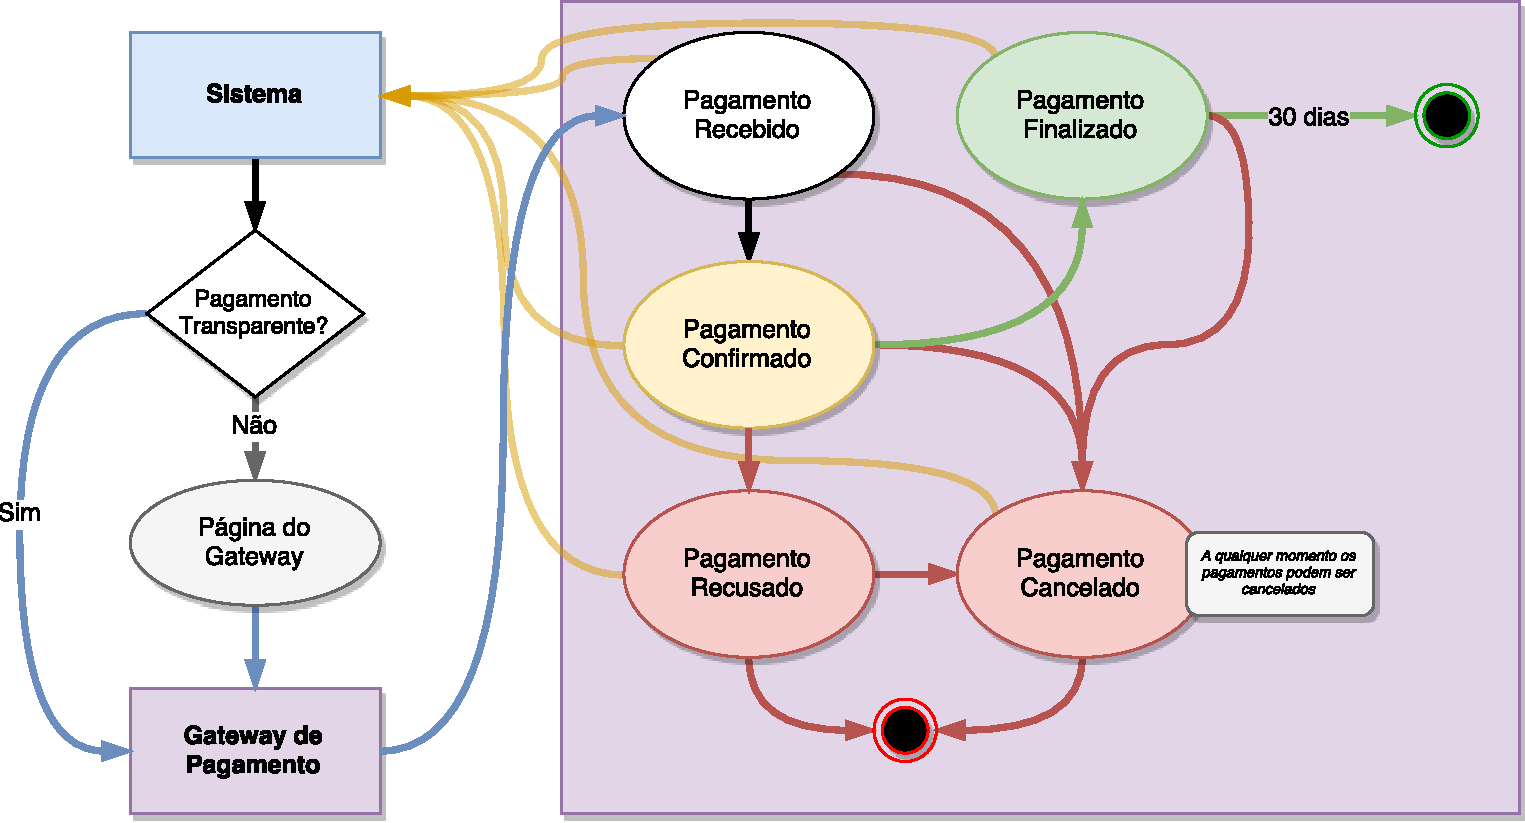
\includegraphics[scale=0.58]{imagens/Processo_Gateway_02.pdf}
    \legend{Fonte: Elaborado pelo Autor}
\end{figure}




\section*{Resumo}
Neste capítulo foi apresentada uma contextualização sobre o problema tratado neste trabalho e a justificativa de tal assunto, que pode-se resumir como sendo necessidade de uma alternativa moderna e simplificada para captação de recursos para ONGs. Ao final, foram detalhados os objetivos gerais e específicos do trabalho.

Os próximos capítulos estão organizados da seguinte forma:

\begin{itemize}
  \item \textbf{Conclusão:} Nesta seção é feita a conclusão do trabalho dado seus objetivos propostos.
  \item \textbf{Trabalhos Futuros:} Nesta seção são listados os trabalhos futuros para melhorar e/ou expandir a utilização da solução.
\end{itemize}